% !TEX root = Entwurf_goApp.tex
\section{Sequenzdiagramme}

\subsection{Benutzer zur einer Gruppe hinzufügen}
Im folgenden werden wir anhand einer Beispiel Funktionalität der goApp interne Abläufe vorstellen.
Im Beispiel geht es darum einen Benutzer der zuvor eine Beitrittsanfrage an eine Gruppe gestellt hat in die Gruppe aufzunehmen.
Hierzu muss der Gründer der Gruppe von der Startseite (StartActivity) zur Gruppeninformationsansicht (GroupInfoActivity) navigieren und dort mit einem Klick die Anfrage bestätigen.
Innerhalb der Datenbank muss hierfür der anfragende Benutzer in die Gruppe hinzugefügt werden und die Beitrittsanfrage anschließend gelöscht werden.
\ \\
\ \\
\ \\
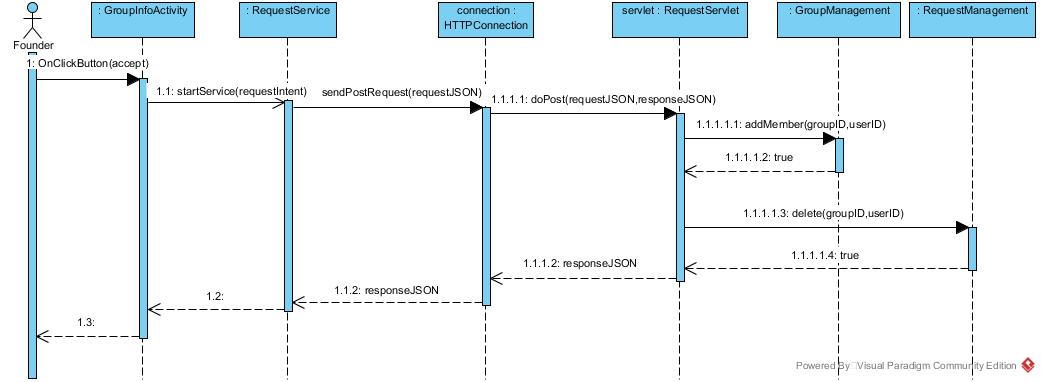
\includegraphics[width=1.1\textwidth]{addMemberSequenceDiagram.jpg}
\ \\
\ \\
Obiges Diagramm veranschaulicht grob wie diese Funktionalität in unserer App umgesetzt wird.
Der Gruppengründer befindet sich hier schon in der GroupInfoActivity und drückt dort den Button um die Anfrage anzunehmen.
Die GroupInfoActivity startet daraufhin mit einem Intent den RequestService, welcher sich um jegliche Bearbeitung von Anfragen kümmert.
Der RequestService schickt mithilfe der Klasse HTTPConnection die Anfrage an das RequestServlet, welches das Gegenstück zum RequestService auf dem Server darstellt.
Die Anfrage wird hier ausgewertet und mithilfe der Klassen welche für die Datenbankverwaltung zuständig sind umgesetzt, in diesem Fall fügt die Klasse GroupManagement den Benutzer in die Gruppe hinzu und die Klasse RequestManagement löscht die Anfrage da diese nicht mehr benötigt wird.
Das RequestServlet antwortet daraufhin dem Clienten und der RequestService sorgt dafür dass der Benutzer über die View ein Feedback bekommt. \newline
Dieses Diagramm zeigt nicht alle Feinheiten der internen Abläufe sondern vereinfacht vieles, es eignet sich aber um einen ersten Überblick zu erhalten.
Die folgenden Diagramme, Activity-Service Kommunikation, Service-ServerConnection Kommunikation und Servlet-Datenbankmanagement Kommunikation illustrieren deshalb die selbe Anfrage, einen Benutzer der zuvor eine Beitrittsanfrage an eine Gruppe gestellt hat in die Gruppe aufzunehmen, detaillierter und spezifisch auf die jeweilige Kommunikation.

\subsubsection{Activity-Service Kommunikation}

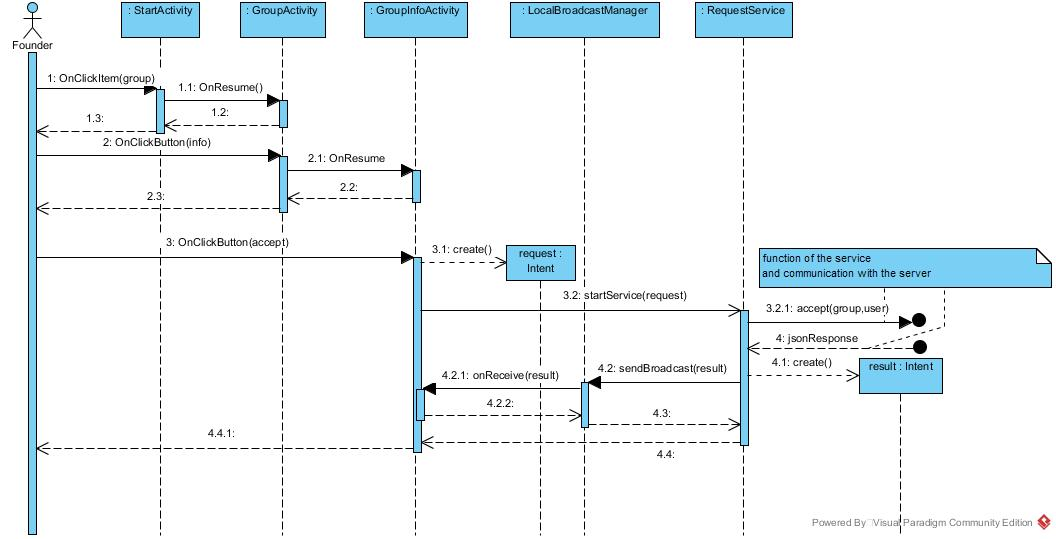
\includegraphics[width=1.1\textwidth]{Activity_Service.jpg}
	

\subsubsection{Service-ServerConnection Kommunikation}
Wenn bei dem RequestService die accept Methode aufgerufen wird, erstellt dieser zunächst ein JSONObject, in dem die Serveranfrage codiert wird. Er fügt dem JSONObject
\begin{itemize}
\item  die ID der Anfrage,
\item den Namen der Methode, welche auf dem Servlet aufgerufen werden soll,
\item die ID der Gruppe, zu der die Gruppenanfrage gehört und
\item die ID des Users welcher in die Gruppe aufgenommen werden will hinzu.
Zusätzlich erstellt der Service eine HTTPConnection und übergibt ihr den Namen des Servlets, an welches die Anfrage geschickt werden soll.
Danach holt er sich von dem JSONObject den JSON-String, in dem die zuvor hinzugefügten Daten enthalten sind. Den übergibt er der Methode sendPostRequest des Klasse HTTPConnection.
Diese sendet dann die Anfrage an den Server, welcher die Anfrage bearbeitet (\hypertarget{ServletDatenbank}{siehe Servlet-Datenbankmanagement Kommunikation}). Der Server sendet ein JSON-String als Antwort zurück, aus welchem die sendPostRequest-Methode ein JSONObject erzeugt und dieses an den RequestService zurück gibt.
%TODO brauchen wir AnfrageID überhaupt
\end{itemize}
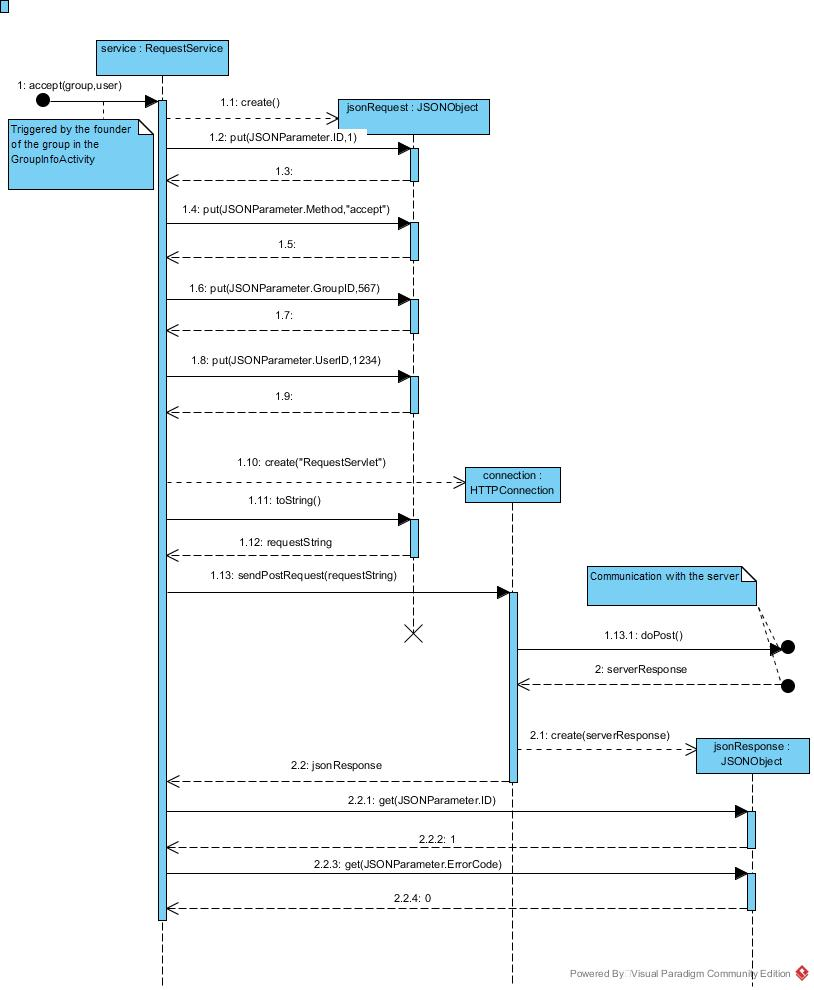
\includegraphics[width=1.1\textwidth]{Service_ServerConnection.jpg}


%Der RequestService erstellt daraufhin einen JSONString und leitet diesen an die Klasse %HTTPConnection weiter, diese Klasse liegt im  Package serverConnection und ist der einzige %Kommunikationsweg der App mit dem Server.
%HTTPConnection wählt das Request Servlet aus und startet auf diesem die passende Methode.
%Von hier werden 


\hyperlink{ServletDatenbank}{}
\subsubsection{Servlet-Datenbankmanagement Kommunikation}

\includegraphics[width=1.1\textwidth]{Servlet_MAnagement.jpg}


\subsection{Clustering Algorithmus}
	
	\newpage